\documentclass[14pt]{beamer}
\title[BPT:VCS:01]{SQL:: MTS\_01}
\author[TS]{TalentSprint}
\institute[L\&D]{Licensed To Skill}
\date{Version Pro 2.0}
\usetheme{Madrid}
\graphicspath{{../Images/}}
\usebackgroundtemplate{
\includegraphics[width=\paperwidth]{TS-XP-Logo.jpg}}
%\graphicspath{{/home/tsuser/Desktop/Latex_Slides/Images/}}

%\graphicspath{{Images/} {ScreenShots/}}

\begin{document}
\begin{frame}
  \titlepage
\end{frame}

\begin{frame}{SQL}
Normalize the below table using the instructions listed below:
 \begin{itemize}
  \item Every attribute has Atomic Value.
  \item Identify the primary key from the available candidate keys.
  \item There are no repeating groups.
  \item Identify the partial dependencies if exist, and eliminate them.
  \item Identify the transitive dependencies if exist, and eliminate them.
 \end{itemize}
\end{frame}

\begin{frame}{SQL}
\begin{center}
    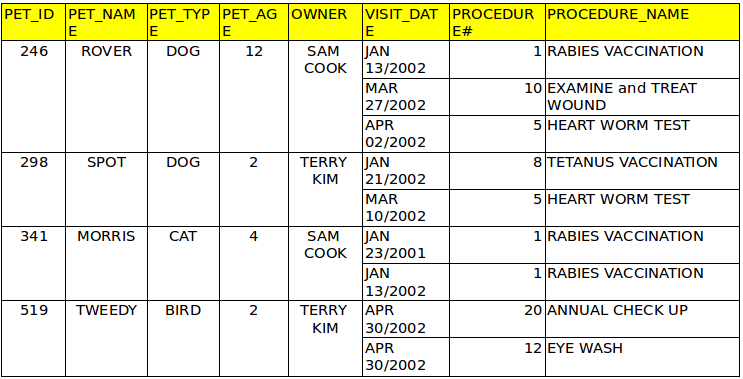
\includegraphics[scale=0.4]{Sql_Image.png}
  \end{center}
\end{frame}

\begin{frame}{SQL}
Draw the Entity relationship diagram.
 \begin{itemize}
  \item Represent the degree (Unary, Binary and Ternary) of relationship existing among tables/entities.
  \item Represent the cardinalities (1-1, 1-N or N-1, N-N) existing between the tables/entities.
  \item Represent the primary key from the identified candidate keys.
  \item Represent the Foreign key if applicable for the table/entity.
 \end{itemize}
\end{frame}
\end{document}

